%Dihiggs physics is cool. Also complicated but not that complicated. Mostly just rare. Show some diagrams. Talk about rates.
\section{Di-Higgs Physics}
\subsection{Double Higgs Production}
\label{sec:physics}

The Higgs boson is an essential part of the Standard Model (SM) of particle physics and is a product of the mechanism responsible for electroweak symmetry breaking. Along with the interaction of the Higgs with the other particles of the Standard Model, the SM predicts the interaction of the Higgs boson with itself at tree-level (self-interaction). This mechanism contributes to non-resonant Higgs boson pair production together with quark-loop contributions via Yukawa-type interactions. Figure~\ref{fig:nr_hh_production} shows a schematic diagram of non-resonant Higgs boson pair production. Since the production cross section for Higgs boson pair production is extremely small within the SM~\cite{deFlorian:2016spz}, 

\begin{equation*}
\sigma_{hh}\text{ (14 TeV)} = 45.1 \text{ fb},
\end{equation*}

any significant deviation would indicate the presence of new physics.

\begin{figure}[!h] 
\begin{center}
\includegraphics*[width=0.75\textwidth] {dihiggsPhys/figures/nr-diHiggs-production.png}
\caption{Leading order Feynman diagrams for non-resonant production of Higgs
  boson pairs in the Standard Model through (a) the Higgs boson self-coupling
  and (b) the Higgs-fermion Yukawa interaction.} 
  \label{fig:nr_hh_production}
\end{center}
\end{figure}

Many extensions of the SM predict the existence of additional scalar bosons which may have mass larger than twice the Higgs mass and can decay into a Higgs boson pair. Searching for resonances in the $hh$ mass spectrum can help us discover or limit exotic models which predict the presence of such particles. More importantly, measuring the SM di-Higgs cross-section (or placing limits on its magnitude) allow us to probe the self-coupling of the Higgs field and better understand the mechanism behind electroweak symmetry breaking.

The following work is focused on techniques for distinguishing non-resonant (SM-like) Higgs boson pair production where both Higgs bosons decay via $h \to b \bar{b}$. The choice of using the $4b$ decay mode provides the largest possible amount of signal events but requires powerful background reduction techniques due to the large production cross-section of fully hadronic QCD processes. All results are quoted for simulated events produced by $pp$ collisions with a center-of-mass energy of 14 TeV and scaled to the full design luminosity of the HL-LHC (an integrated luminosity of 3000 fb$^{-1}$). Simulated samples were produced using ROOT v6.12/04~\cite{Brun:1997pa} and Madgraph v2.7.0~\cite{Alwall:2014hca}. Events were then showered using Pythia v8.2.44~\cite{Sj_strand_2015} and reconstructed with Delphes v3.0~\cite{de_Favereau_2014} using the v2 approximation of the upgraded Phase-II CMS detector.

Both the signal and background samples were generated with minimal pileup addition sampled from a Poisson distribution with an expectation value of zero additional vertices. An additional generator-level cut requiring total hadronic energy greater than 300 GeV was applied when generating background events. All code used to set up the generation environment and produce events is publicly available~\cite{github}. A summary of the sample generation details is shown in Table~\ref{tab:samples}.

\begin{table}[ht!]
 \label{tab:samples}
\centering
  %\begin{center}
    \begin{tabular}{|l|c|c|c|} % <-- Alignments: 1st column left, 2nd middle and 3rd right, with vertical lines in between
      \hline\hline
      Name & Process & $\sigma_{\textrm{eff}}$ [fb] & $N_{\textrm{events}}$ \\
      \hline
      Di-Higgs & $p p > h h$, $h > b \bar{b}$ & 12.4 & 1$\cdot 10^6$ \\
      QCD     & $p p > b \bar{b} b \bar{b}$ & 441866.0 & 4$\cdot 10^6$ \\
      \hline\hline
    \end{tabular}
\caption{Madgraph processes, effective cross-sections, and number of generated events for the signal and background samples used in this paper. The effective cross-sections differ slightly from the total theoretical cross-sections due to branching fractions and generation-level cuts on hadronic activity.}
\end{table}

\subsection{Event Reconstruction}
\label{sec:eventReco}
The first step in reconstructing the 4$b$ system is to reconstruct and select b-jet candidates. Jets are clustered using an anti-$k_T$ algorithm with a radius of R=0.4. To be selected for use in event reconstruction, a jet must have $\pt > 20$ GeV and an absolute value of $\mid\eta\mid < 2.5$. Delphes uses an internal $b$-tagging efficiency parameterization to predict whether jets are tagged, and an event is only fully reconstructed if at least 4 jets are $b$-tagged (unless otherwise specified). The properties and kinematics of selected jets are shown in Fig~\ref{fig:jetInfo}. This strict requirement of having at least 4 $b$-tags in an event helps to reduce contributions from QCD and reduce the combinatoric ambiguity in event reconstruction.

\begin{figure}[ht!]
  \begin{center}
  \subfloat[]{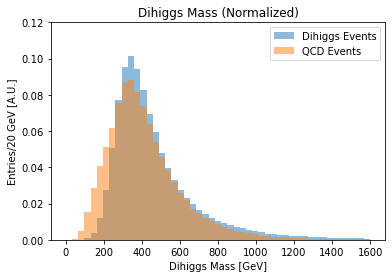
\includegraphics[width = 2in]{dihiggsPhys/figures/recoPlots_08-21-20/dihiggs_DihiggsMass_norm}} 
  \subfloat[]{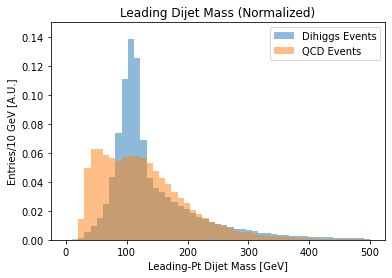
\includegraphics[width = 2in]{dihiggsPhys/figures/recoPlots_08-21-20/leading_Leading-PtDijetMass_norm}}
  \subfloat[]{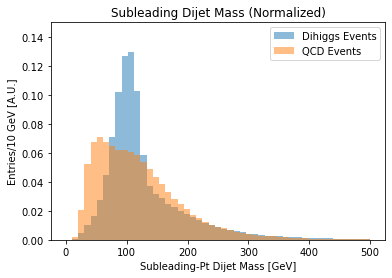
\includegraphics[width = 2in]{dihiggsPhys/figures/recoPlots_08-21-20/subleading_Subleading-PtDijetMass_norm}}\\
  \subfloat[]{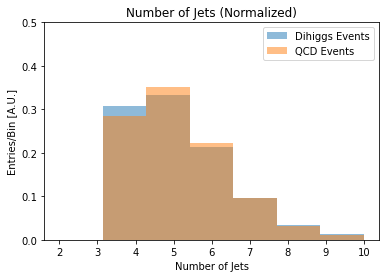
\includegraphics[width = 2in]{dihiggsPhys/figures/recoPlots_08-21-20/number_NumberofJets_norm}}
  \subfloat[]{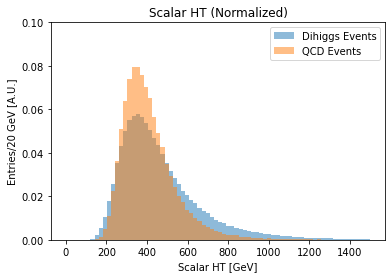
\includegraphics[width = 2in]{dihiggsPhys/figures/recoPlots_08-21-20/scalar_ScalarHT_norm}}
  \subfloat[]{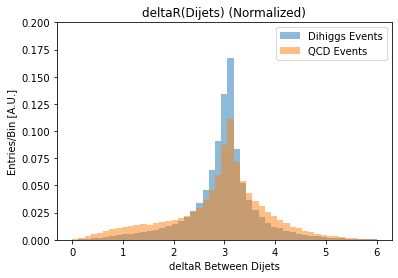
\includegraphics[width = 2in]{dihiggsPhys/figures/recoPlots_08-21-20/deltar(dijets)_deltaRBetweenDijets_norm}} 
  \caption{Sample of event kinematics and reconstructed di-Higgs system from QCD and di-Higgs simulation. Distributions are normalized to the same area to compare shapes.}
  \label{fig:jetInfo}
  \end{center}
\end{figure}

Once events with at least 4 $b$-tags are selected, there is a choice about how to reconstruct the di-Higgs system. Several reconstruction methods were tested for pairing b-jets to find an optimal algorithm for correctly pairing Higgs boson constituents. Two algorithms were selected for use in the following sections: the first iterates through all selected jets in an event and returns the two pairs with closest di-jet masses to one another and the second returns the two jet pairs that minimize the difference between the individual candidate pairs and a Higgs boson mass of 125 GeV. Unless otherwise specified, the method that selects di-jets with masses closest to each other is used when training techniques that require reconstructed events. Fig~\ref{fig:jetInfo} shows a selection of distributions describing the di-Higgs system using this reconstruction algorithm.% Figure~\ref{fig:comapreReco} compares the dijet pair masses obtained from both algorithm. 

%\begin{figure}[ht!]
%  \begin{center}
%  \subfloat[]{\includegraphics[width = 2.5in]{dihiggsPhys/figures/reconstructedQuantities/mh_pairJetsUsingSmallestDeltaR}} 
%  \subfloat[]{\includegraphics[width = 2.5in]{dihiggsPhys/figures/reconstructedQuantities/mh_pairJetsClosestToHiggs}}\\
%  \caption{Leading dijet mass using different reconstruction algorithms. Left plot shows mass when minimizing dijet angular separation, right plot shows mass when minimizing different between dijet mass and a Higgs mass of 125 GeV ('closestDijetMassToHiggs'). [PLACEHOLDER PLOTS]}
%  \label{fig:compareReco}
%  \end{center}
%\end{figure}

Reconstructed variables include the masses and momentum of the four- and two-body Higgs candidates as well as the angular separations between the two Higgs candidates and their constituent jets. Additional event-level variables like the number of selected jets, the number of b-tagged jets, and the missing transverse energy in the event were also considered as inputs to various algorithms. All possible variables were evaluated using the Kolmogorov-Smirnov (KS) test for individual separation power between signal and background. Variables were sorted in descending order of KS separability. Each algorithm is trained on a subset that balances minimizing the number of variables without sacrificing performance. 
